%Latex->PDF
%
% TRUCJE (afhankelijk van de bestandsnaam, krijg je de handout of de presentatie ...
% (!! GEBRUIK LINUX HARD LINKS OM HETZELFDE BESTAND TWEE NAMEN TE GEVEN !!)
% See https://tex.stackexchange.com/questions/197330/how-can-i-check-if-the-filename-of-a-latex-document-contains-a-string
%
\RequirePackage{substr}   % RequirePackage omdat \usepackage niet werkt voor \begin{document} !

\begingroup\escapechar=-1
\xdef\handoutstring{\string\handout}   % dirty hack, omdat anders stringcompare niet werkt
\endgroup

\IfSubStringInString{\handoutstring}{\jobname}
{
\documentclass[handout]{beamer}
\wlog{We genereren de HANDOUT versie voor \jobname.}
}{
\documentclass{beamer}
\wlog{We genereren de PRESENTATIE versie voor \jobname.}
}
% EndofTrucje


\usepackage[dutch]{babel}
\usepackage{amssymb,amsmath,amsthm}

\usepackage{cancel}
\usepackage{relsize}

\usepackage{listings}
\usepackage{xcolor}
%\usepackage{verbatim}

\setbeamertemplate{headline}{\insertframenumber/\inserttotalframenumber}
\newcommand{\ds}{\displaystyle}
\newcommand{\N}{\ensuremath{\mathbb{N}}}
\newcommand{\Z}{\ensuremath{\mathbb{Z}}}
\newcommand{\Nnul}{\ensuremath{\mathbb{N}_0}}
\newcommand{\Q}{\ensuremath{\mathbb{Q}}}
\newcommand{\R}{\ensuremath{\mathbb{R}}}
\newcommand{\perdef}{\overset{\mathrm{def}}{=}}
\newcommand{\Bgsin}{\mathrm{Bgsin}\,}
\newcommand{\Bgcos}{\mathrm{Bgcos}\,}
\newcommand{\Bgtan}{\mathrm{Bgtan}\,}

\DeclareMathOperator{\dom}{dom}     % domein
\DeclareMathOperator{\codom}{codom} % codomein
\DeclareMathOperator{\bld}{bld}     % beeld
\DeclareMathOperator{\graf}{graf}   % grafiek
\DeclareMathOperator{\rico}{rico}   % richtingcoëfficient
\DeclareMathOperator{\co}{co}       % coordinaat

\newtheorem*{eigenschap}{Eigenschap}

\newcommand{\p}{\pause}
\newcommand{\important}[1]{\ensuremath{\colorbox{lightgray}{$#1$}}}

\providecommand{\blue}[1]{{\color{blue}#1}}  
\providecommand{\red}[1]{{\color{red}#1}}  

\usepackage{pgf,tikz,pgfplots}
%\pgfplotsset{compat=1.15}
\usepackage{mathrsfs}
\usepackage{dsfont}
\usepackage{relsize}   % voor \mathlarger
\usetikzlibrary{arrows}
 \usepgfplotslibrary{fillbetween}
 \usetikzlibrary{positioning, fit, calc} 
 \usetikzlibrary{intersections}
 \usetikzlibrary{shapes}
%\pagestyle{empty}

\title{Ximera}
\subtitle{TUG2024}
\author{Wim Obbels}
\date{July 19 2024}
\usetheme{CambridgeUS}
\usecolortheme{seahorse}

\usepackage{rawfonts}
%\input{prepictex}
%\input{pictex}
%\input{postpictex}

\graphicspath{
	{../../}
	{../}
	{./}
  	{../../pictures/}
   	{../pictures/}
   	{./pictures/}
}

\begin{document}

\tikzset{block/.style={draw, thick, text width=3cm , minimum height=2cm, % align=center,
     rectangle split, 
     rectangle split ignore empty parts, 
     rectangle split parts=3,
     rectangle split part align={center, left},
     rounded corners=0.2cm,
     draw},   
     line/.style={-latex}     
}  

  

% %\pdfOnly{\begin{landscape} }
  
% \begin{image}[\textwidth]
% \begin{tikzpicture}  

% \node[block, fill=green] (pceind) {
%           PC Eindgebruiker
%           \nodepart{two}
%           - browser
%          };  


% \node[block, fill=orange!50!white, below=of pceind ] (pc1) {
%     PC Auteur 1
%     \nodepart{two}
%     - browser \\          
%     - git client\\ 
%     - docker client
%     \nodepart{three} Repositories:\\
%     - clone cursus1.tex    
%     }; 

% \node[block, fill=orange!50!white, below=0.2cm of pc1 ] (pc2) {
%     PC Auteur 2
%     \nodepart{two}
%     - browser \\          
%     (via Gitlab IDE)
% }; 


% \node[block, fill=orange!50!white,below=0.2cm of pc2  ] (pc3) {
%     PC Auteur 3
%     \nodepart{two}
%      - browser \\
%      - git client\\ 
%      - LaTeX client
%     \nodepart{three} Repositories:\\
%     - clone cursus1.tex \\
%     - clone ximera.cls
%     };  

     
% \node[block,right=of pceind, fill= green,text width=11.5cm] (ximeraserver) {
%   Ximera Server (publieke website, via de ICTS Cloud en docker)
%   \nodepart{three} \url{set.kuleuven.be/voorkennis/zomercursus}
%   };  
% %
% \node[block, below right=2cm of pceind, fill=orange,text width=5cm ] (gitrunner) {  % geknoei
%     GITLAB runner
%     \nodepart{two}
%     Genereert PDF en HTML \\
%     naar Ximera Server (xake)
% }; 

% \node[block, right=of gitrunner, fill=orange,text width=5cm] (elsschot) {
%     Cloud Management (docker)
%     \nodepart{three} \url{elsschot.icts.kuleuven.be}
% };  


% \node[block, fill=orange!50!white,below =of gitrunner,text width=5cm     ] (gitrepo) {
%   GITLAB Repository server
%   \nodepart{two}
%     met git-repositories ((broncode):\\
%     - repo cursus1.tex\\
%     - repo cursus2.tex\\
%     - repo ximera.cls\\
%     - repo ximeraserver.js\\
%     - repo xake.go\\
%     - repo gitlabrunner.docker\\
%    updates publiceren via GITLAB runner\\
%    webpagina's beheer/diagnose\\ 

%     \nodepart{three}
%        \url{gitlab.kuleuven.be}
%     };  


% \node[block, right=of gitrepo, fill=orange,text width=5cm ] (dockerrepo) {
%     Docker Repository Server \\
%     ( Artifactory / FROG )
%     \nodepart{two}met docker images \\
%     - ximeraserver\\
%     - xake\\
% %    - gitlabrunner
%     \nodepart{three} \url{repo.icts.kuleuven.be}
% };  


% %\node[block, fill=orange , below=of pceind ] (pcbeheer) {
%     \node[block, fill=orange , below right=of ximeraserver] (pcbeheer) {
%         PC Beheerder
%         \nodepart{two}
%         - browser \\          
%         - git client\\
%         - docker client
%         \nodepart{three} Repositories:\\
%         - clone ximeraserver \\
%         - clone gitlabrunner
%     };  
    


  
% % Kader ICTS 

% \node[draw, fill=gray, fill opacity=0.1,inner xsep=5mm,inner ysep=6mm,
%       fit=(ximeraserver)(dockerrepo)(elsschot)(gitrepo)(gitrunner),
%       label={90:ICTS Cloud / SET-IT}] (icts) {};   

% % Connecties ...
% \draw[line,->] (pceind)-- (ximeraserver);  
          
% \draw[line,<->] (pc2) -- (pc2-|gitrepo.west);  
% %\draw[line,<->] (pc1) -- (pc1-|gitrepo.west); 
% \draw[line,<->] (pc3) -- (pc3-|gitrepo.west);  
% \draw[line, ->,very thick,orange!50!white] (pc1.south east) -- node[black,above]{update} (gitrepo.north west);
% %\draw[line, ->] (pc2.north east)-- (ximeraserver.west);

% \draw[line,<-,very thick, orange]  (ximeraserver.south-|elsschot) -- node[black,right]{beheer} (elsschot); 
% \draw[line,<->] (elsschot) -- (dockerrepo); 

% \draw[line,->] (pcbeheer) |- (ximeraserver.east);  
% \draw[line,->] (pcbeheer) |- (dockerrepo.east);  
% \draw[line,->] (pcbeheer) -- (elsschot);  
% \draw[line,->] (pcbeheer.210) -- (gitrepo.north east);  

% \draw[line,->,very thick,orange!50!white] (gitrunner)                -- node[black,right,pos=0.5]{update} (gitrunner.north |- ximeraserver.south);  
% \draw[line,->,very thick,orange!50!white] (gitrunner.south-|gitrepo) -- node[black,left]{pull} 
% (gitrepo); 
% \draw[line,-> ] (gitrunner.south-|dockerrepo) -- (dockerrepo);  

% % Legende
% \node[block, fill=orange!50!white,below =4cm of pcbeheer  ] (la) {Voor Auteurs};
% \node[block, fill=orange,         below=0.1cm of la         ] (lb) {Voor Beheerders};
% \node[block, fill=green ,         above=0.1cm of la         ] (lb) {Voor Eindgebruikers};

% \end{tikzpicture}  
% \end{image}



\begin{frame}
  \titlepage
\end{frame}


\begin{frame}[t]{\Large\blue{Ximera}}

  \begin{itemize}
  \item is pronounced \lq chimera\rq
  \item stands for \\
     {\Large\blue X}imera: {\Large\blue I}nteractive {\Large\blue M}athematical {\Large\blue E}ducational {\Large\blue R}esources for {\Large\blue A}ll
  \item is an open-source platform 
  \item supports authoring and publishing interactive educational content
  \item such as worksheets, assessments, textbooks and online courses. 
  \item both in PDF and Online
  \item authors only write \LaTeX %, most \LaTeX constructs are supported
  \end{itemize}
   
  \vfill

  The ultimate goal: promote sustained student success and savings.
  
  % The Ximera Project is funded 2024-2026 with (no other external funding) by a $2,125,000 Open Textbooks Pilot Program grant. In the past, the Ximera Project has also recieved support from NSF Grant DUE-1245433, the Shuttleworth Foundation, the Ohio State University Department of Mathematics, and the Affordable Learning Exchange at OSU. 
  

\end{frame}

\begin{frame}[t]{Intro}
  
%  \providecommand{\answer}[1]{\blue{#1}}
% \begin{enumerate}
%     \item $\mu$     (presumed population mean)      = $\answer{400}$
%     \item $\sigma$  (population standard deviation) = $\answer{25}$
%     \item $\bar{x}$ (sample mean)                   = $\answer{410}$
%     \item $n$       (sample size)                   = $\answer{100}$
% \end{enumerate}
%   \begin{lstlisting}
%     hallo 
% \end{lstlisting}

\begin{center}
  \resizebox{0.6\linewidth}{!}{
    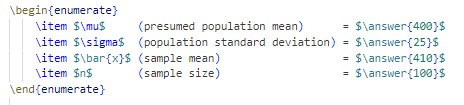
\includegraphics{SimultaneousOutputSource.jpg}
  }  
  \vfill
  \resizebox{0.8\linewidth}{!}{
    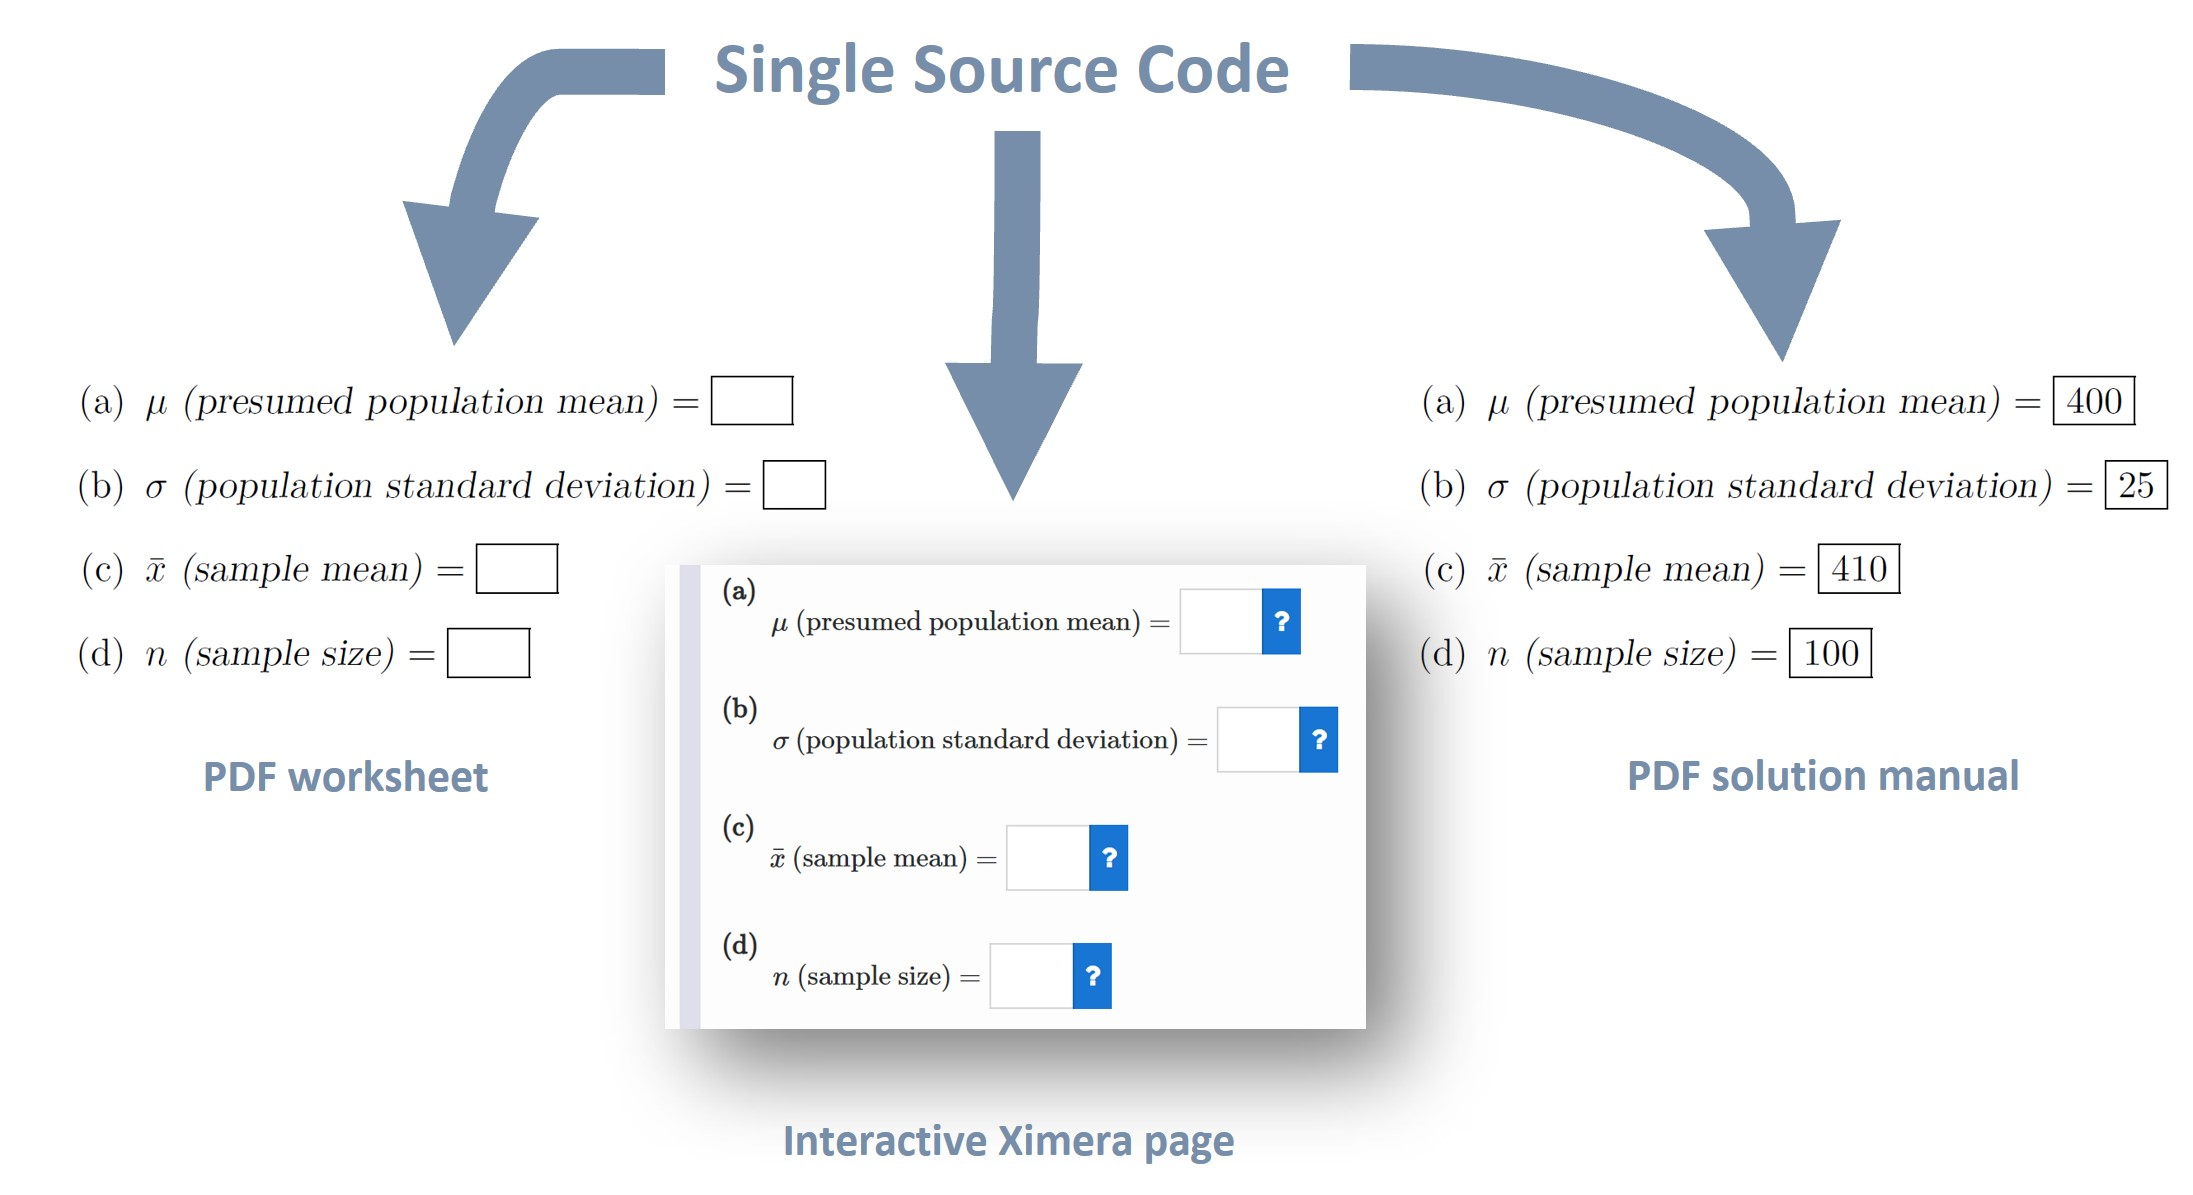
\includegraphics{SimultaneousOutput.jpg}
  }
\end{center}

\end{frame}
\begin{frame}[t]{Styling (HTML/PDF)}
  
\begin{center}
  \resizebox{\textwidth}{!}{
    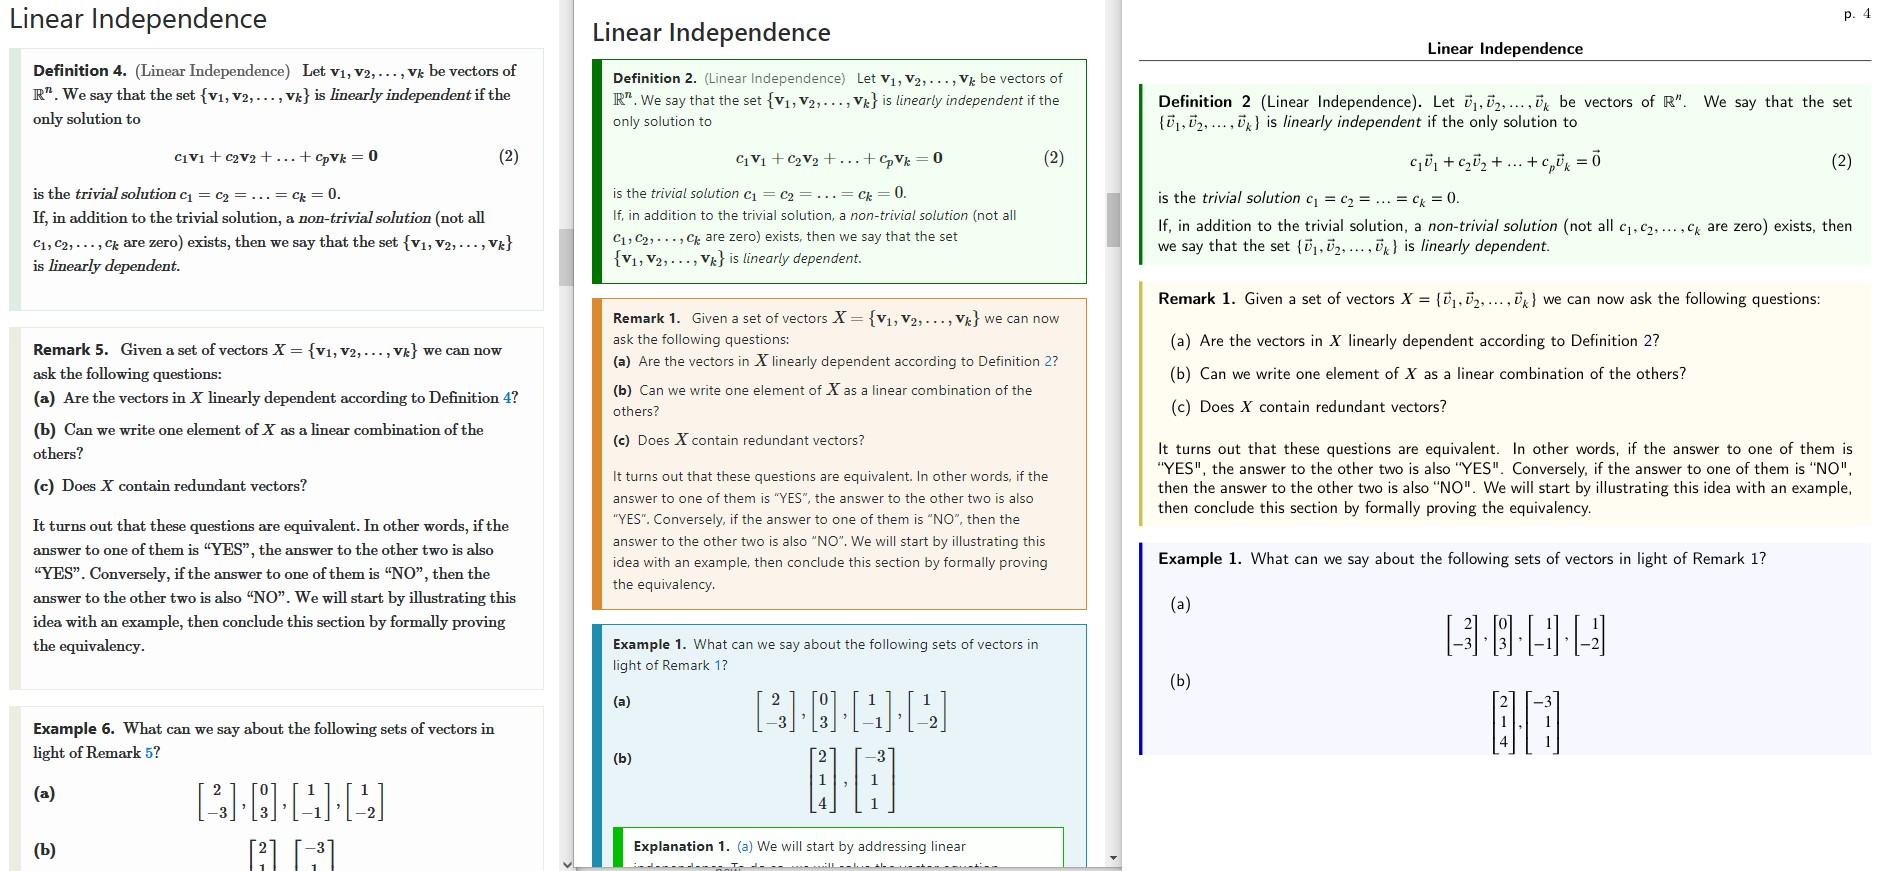
\includegraphics{Styling_LinearIndependence.jpg}
  }  

\end{center}

\end{frame}

\begin{frame}[t]{Build Architecture ('classic')}

  \resizebox{\linewidth}{!}{
\begin{tikzpicture}  

\node[block, fill=green,text width=6cm] (pcenduser) {
          PC Enduser
          \nodepart{three}
          - browser
};  

\node[block,right=of pcenduser, fill= green,text width=10cm] (ximeraserver) {
          Ximera Server (public website)
          \nodepart{three} 
          \url{https://ximera.osu.edu}\\
          \url{https://set.kuleuven.be/voorkennis}
};          

\node[block, fill=orange!50!white,below=1cm of pcenduser, text width=6cm ] (pcauthor) {
    PC Author (classic)
    \nodepart{two}
    - \LaTeX installation \\
    - git client \\ 
    - editor \\
    - GPG key \\
    - xake \\
    - browser
    \nodepart{three} Procedure:\\
    - git clone course.git \\
    - edit \LaTeX code \\
    - git commit \\
    - xake bake/frost/serve
};  

\draw[line,->] (pcenduser) -- node[above] {} (ximeraserver);  
          
\draw[line,->] (pcauthor) -- node[right] {xake (https PUT)} (ximeraserver);  

\node[draw, fill=gray, fill opacity=0.1,inner xsep=5mm,inner ysep=6mm,
      fit=(ximeraserver),
      label={90:Cloud}] (icts) {};   


\end{tikzpicture}
  }

\end{frame}

\begin{frame}[t]{Build Architecture ('local docker')}

\resizebox{\linewidth}{!}{
\begin{tikzpicture}  
\node[block, fill=green,text width=6cm] (pcenduser) {
          PC Enduser
          \nodepart{three}
          - browser
};  

\node[block,right=of pcenduser, fill= green,text width=10cm] (ximeraserver) {
          Ximera Server (public website)
          \nodepart{three} 
          \url{https://ximera.osu.edu}\\
          \url{https://set.kuleuven.be/voorkennis}
};          

\node[block, fill=orange!50!white,below=1cm of pcenduser, text width=6cm ] (pcauthor) {
    PC Author (local docker)
    \nodepart{two}
    - \textbf{docker} \\
    - git client\\ 
    - editor (strong suggestion: VSCode) \\
    - GPG key\\ 
    \phantom{- xake}\\
    - browser
    \nodepart{three} Procedure:\\
    - git clone course.git \\
    - edit \LaTeX code \\
    - git commit \\
    - \textbf{docker} xake bake/frost/serve
};  

\draw[line,->] (pcenduser) -- node[above] {} (ximeraserver);  
          
\draw[line,->] (pcauthor) -- node[right] {xake (https PUT)} (ximeraserver);  

\node[draw, fill=gray, fill opacity=0.1,inner xsep=5mm,inner ysep=6mm,
      fit=(ximeraserver),
      label={90:Cloud}] (icts) {};   


\end{tikzpicture}
  }

\end{frame}


\begin{frame}[t]{Build Architecture ('cloud')}

\resizebox{\linewidth}{!}{
\begin{tikzpicture}  

\node[block, fill=green,text width=6cm] (pcenduser) {
          PC Enduser
          \nodepart{three}
          - browser
};  
\node[block,right=of pcenduser, fill= green,text width=10cm] (ximeraserver) {
          Ximera Server (public website)
          \nodepart{three} 
          \url{https://ximera.osu.edu}\\
          \url{https://set.kuleuven.be/voorkennis}
};          

\node[block, fill=orange!50!white,below=1cm of pcenduser, text width=6cm ] (pcauthor) {
    PC Author (local/cloud docker)
    \nodepart{two}
    - docker \\
    - git client\\ 
    - editor (strong suggestion: VSCode) \\
    \phantom{- GPG key}\\ 
    \phantom{- xake}\\
    - browser
    \nodepart{three} Procedure:\\
    - git clone course.git \\
    - edit \LaTeX code \\
    - git commit \\
    - (optional) docker xake bake \\
    - \textbf{git push}
};  

\node[block, fill=orange!50!white,below =of ximeraserver,text width=10cm     ] (gitrepo) {
  Github/GITLAB Repository server
  \nodepart{two}
    - repo xourse.git \\
    - docker image repository \\
    - GPG Key(s) \\
    - Authentication and Authorization
    \nodepart{two}
    Actions or pipelines do \\
    - xake bakePdf  (with and/or without answers) \\
    - xake bake/frost/serve
    \nodepart{three}
       \url{https://gitlab.kuleuven.be} \\
       \url{https://github.com}
    };  

    \node[draw, fill=gray, fill opacity=0.1,inner xsep=5mm,inner ysep=6mm,
      fit=(ximeraserver)(gitrepo),
      label={90:Cloud}] (icts) {};   



\draw[line,->] (pcenduser) -- node[above] {} (ximeraserver);  
          
\draw[line,->] (pcauthor.320) -- node[below right] {push/pull} (gitrepo);  

\draw[line,->] (gitrepo) -- node[right] {xake} (ximeraserver);  

\end{tikzpicture}
  }

\end{frame}


\end{document}